% !TeX spellcheck = en_US
\documentclass[11pt, a4paper]{article}
\usepackage[utf8]{inputenc}

\usepackage{latexsym}
\usepackage{float}
\usepackage[utf8]{inputenc}
\usepackage[english]{babel}
\usepackage{microtype}
\usepackage[hyphens]{url}
\usepackage{hyperref}
\usepackage{graphicx}
\usepackage{makeidx}
\usepackage{datetime}
\usepackage{multicol}
\usepackage{setspace}
\usepackage{pdflscape}
\usepackage{pgffor}
\usepackage{enumerate}
\usepackage{booktabs}
\usepackage{tabularx}
\usepackage{braket}
\usepackage{listings}
\usepackage{color}
\usepackage{amsmath}
\usepackage{amssymb}
\usepackage[table,xcdraw]{xcolor}
\usepackage{graphicx}
\usepackage{listings}
\usepackage{hyperref}
\usepackage{vmargin}
\usepackage{wrapfig}
\usepackage{subfiles}
\usepackage{float}
\usepackage{amsmath}
\usepackage{amssymb}
\usepackage{tikz-cd}
\usepackage{multirow}
\usepackage{pgffor}
\usepackage{enumitem}
\usepackage{iflang}
\usepackage{varioref}
\usepackage{hyperref}
\usepackage{cleveref}
\usepackage{caption}
\usepackage{subcaption}
\usepackage{tikz}
\usepackage{enumitem}
\usepackage{xpatch}
\usepackage{refcount}
\usepackage{color}
\usepackage{pdfpages}
\usepackage{array}
\usepackage{eurosym}
\usepackage{longtable}

%%%%%%%%%%%%%%%%%%%%%%%%%%%%%%%%%%%%%%%
%%%%%%%%%%%% UTIL COMMANDS %%%%%%%%%%%%  

\setcounter{secnumdepth}{4}
\newcommand{\nc}{\newcommand}
\nc{\supindex}{\textsuperscript}
\renewcommand{\baselinestretch}{1.5}
\nc{\myparagraph}[1]{\paragraph{#1}\mbox{}\\}

%%%%%%%%%%%%%%%%%%%%%%%%%%%%%%%%%%%%%%%
%%%%%%%%%%%%% CONFIG FILE %%%%%%%%%%%%%

\nc{\mytitle}{Game Of Life parallelization with OpenMP}
\nc{\mysubtitle}{Bayesian Inference}
\nc{\authors}{
	Oriol Alàs Cercós,  Sergi Simón Balcells
}
\nc{\datetime}{17\supindex{th} of March, 2022}
\nc{\assignatura}{High Performance  Computing}
\nc{\professorat}{Francesc Giné, Jordi Ricard Onrubia}

% Per separar professors, utilitzar ','
% 	Ex: Maria, Joan, Pere

%%%%%%%%%%%%%%%%%%%%%%%%%%%%%%%%%%%%%%%
%%%%%%%%%%%%%  LANGUAGE   %%%%%%%%%%%%%

\newcommand{\tr}{\IfLanguageName{english}}

%%%%%%%%%%%%%%%%%%%%%%%%%%%%%%%%%%%%%%%
%%%%%%%%%%%%%%%%% MATH %%%%%%%%%%%%%%%%

\nc{\prob}[1]{P({#1})}
\nc{\probl}[2]{P({#1}|{#2})}

%%%%%%%%%%%%%%%%%%%%%%%%%%%%%%%%%%%%%%%
%%%%%%%%%%%%% FUNCTIONS %%%%%%%%%%%%

\nc{\numitems}[1]{\getrefnumber{#1}}
\newcounter{itemcntr}
\AtBeginEnvironment{itemize}{%
	\setcounter{itemcntr}{0}%
	\xapptocmd{\item}{\refstepcounter{itemcntr}}{}{}%
}

%%%%%%%%%%%%%%%%%%%%%%%%%%%%%%%%%%%%%%%
%%%%%%%%%%%%% RADIO BUTTON %%%%%%%%%%%%

\makeatletter
\newcommand*{\radiobutton}{%
	\@ifstar{\@radiobutton0}{\@radiobutton1}%
}
\newcommand*{\@radiobutton}[1]{%
	\begin{tikzpicture}
		\pgfmathsetlengthmacro\radius{height("X")/2}
		\draw[radius=\radius] circle;
		\ifcase#1 \fill[radius=.6*\radius] circle;\fi
	\end{tikzpicture}%
}
\makeatother


%%%%%%%%%%%%%%%%%%%%%%%%%%%%%%%%%%%%%%%
%%%%%%%%%%%%%  %%%%%%%%%%%%


\newcolumntype{S}{>{\centering\arraybackslash}m{1.5em}}

\renewcommand{\tabularxcolumn}[1]{m{#1}} % redefine 'X' to use 'm'
\newcommand{ \titem}[1]{\item \textbf{#1}\quad}

\newcommand{\costVar}[4]{In that moment, we want to earn $\frac{#1\text{€}}{1 h}$, therefore the human resource cost will be: \[#2 \cdot \frac{#3h}{1 day} \cdot \frac{#1\text{€}}{1 h} = #4 \text{€}\] }

\nc{\numbers}[1]{
	\begin{tabularx}{#1\textwidth}{|S|S|S|S|S|}
		\hline 1 & 2 & 3 & 4& 5 \\\hline
	\end{tabularx}
}

\nc{\optionsofcol}{
	\multicolumn{3}{c}
	{%
		\numbers{0.338}
	}
}

\nc{\options}{\multicolumn{2}{c}
	{%
		\numbers{0.338}
}}


\newcolumntype{P}[1]{>{\centering\arraybackslash}p{#1}}

\setpapersize{A4}

\author{Oriol Alàs Cercós}
\date{29 d'Abril del 2019}

\def\contentsname{Índex}
\begin{document}
	
	\definecolor{gray}{rgb}{0.4,0.4,0.4}
	\definecolor{darkblue}{rgb}{0.0,0.0,0.6}
	\definecolor{cyan}{rgb}{0.0,0.6,0.6}
	\lstset{
		basicstyle=\ttfamily,
		columns=fullflexible,
		showstringspaces=false,
		commentstyle=\color{gray}\upshape
	}
	
	\lstdefinelanguage{XML}
	{
		morestring=[b]",
		morestring=[s]{>}{<},
		morecomment=[s]{<?}{?>},
		stringstyle=\color{black},
		identifierstyle=\color{darkblue},
		keywordstyle=\color{cyan},
		morekeywords={xmlns,version,type}% list your attributes here
	}
	
	\begin{titlepage}
		\begin{figure}[htb]
			\begin{center}
				
				\includegraphics[width=5cm]{imgs/udl.png}\\
				
				
				\medskip
				\begin{center}
					
					\huge\textbf{\mytitle}\\
					\bigskip
					\normalsize{\tr{Made by}{Realitzat per:}}
					\\
					\large\textit{\authors}
					\\
					\setlength{\parskip}{1em}
					\normalsize{\tr{Delivery}{Data de lliurament:}}
					\\
					\large{\datetime}
				\end{center}
				
				\vspace*{\stretch{2.0}}
			\end{center}
		\end{figure}
		\begin{flushright}
			Universitat de Lleida
			\\
			Escola Politècnica Superior
			\\
			Màster en Enginyeria Informàtica
			\\
			\assignatura
			\\
			\medskip
			\textbf{\tr{Professorate:}{Tutor:}}
			\\
			\foreach \n in \professorat{\n\\}
		\end{flushright}
		\thispagestyle{empty} 
	\end{titlepage}
	\tableofcontents
	\listoftables
	\listoffigures
	\thispagestyle{empty}
	\thispagestyle{empty}
	\newpage
	\section{Introduction}
	In this project, it will be discussed how we have parallelized the code of the game of life provided by the professors. First, we will talk about the design choices that were done during the development, as well as some changes that were made to the sequential code to make the analysis of speed up and efficiency more true to the game of life.\\
	\\
	Then, we will provide the results of this code executed at the Moore cluster with the examples of 5000 and 10000 matrices provided in the assignment. In the same section, we will analyze why the application behaves like that.\\
	\\
	Finally, a conclusion to the analysis is provided, where we remark on the key points that were discovered in the analysis.
	
	\section{Design Choices}
	% loops parallelized
	% removed file writing
	% different types of schedules tried
	% with optimization 3
	% change in parameters from the execution
	There are 6 loops parallelized on the modified code that was given by the professors. The first two that could appear in the code are for generating randomly the grid with the given parameters. It may be weird to see it is only this kind of loop that is parallelized, but reading data from a sequential disk concurrently only makes it gain little to no speedup and brings down the efficiency of the data is not processed extensively. In our case, as it is a simple assignment to our grid variable, it only makes it perform worse. \\
	\\
	The next two loops correspond to the update of the grid for each step. The first is for computing a second grid that counts how many cells are alive. This makes the second be able to compute easily and faster if the cell will be dead or alive. The last two loops correspond when a grid is read from a file, as there are two loops in this step to set the borders of the grid to dead.\\
	\\
	Moreover, There were some changes made to the serial code that was provided by the professor. The code wrote the steps for checking the application in the main loop. As said before, writing in a file system is costly as it can only be done sequentially as well as is slower than the CPU capacity. For this reason, we made the steps stored for debugging an optional activated by the constant debug. This was made solely to study better the speedup and efficiency of the program.\\
	\\
	There was a decision that was left to be empirically demonstrated between different executions, which was which type of schedule should the application use. We tried to do it dynamically, statically, and with guiding policies. The dynamically and statically performed badly in comparison to the guided one, with the statically even worsening with the number of cores to parallelize. Nevertheless, the guided strategy performed better than all of them, and, as we will see in the analysis, the efficiency and the speed-up with different cores are almost linear.
	\\
	\\
	In addition, the code was compiled with \texttt{-O3} flag from the GCC to activate the optimizations. It performs an order of magnitude better than the code not optimized. This is not surprising as the loop contains an if-else that sets the boolean condition for the cell to be alive or dead. With the \texttt{branchless} optimization, most of the statements inside a loop are removed in favor of multiplication to set the variable inside them. This means that the hardware can compute more efficiently the instructions, and, as said, Game of Life makes extensive use of this optimization.\\
	\\
	Finally, was added a parameter to the execution. The full execution is:
	
	\begin{verbatim}
    lifegame cores [name-of-file] [x-size] [y-size] [max-iterations]
	\end{verbatim}
This lets us make it easier to execute the application in the backend without needing to recompile it each time.
	\section{Results}
	The results are gathered in the table \ref{tab:time} \ref{tab:speedup}, \ref{tab:efficiency}. There are different graphics that can be seen in these application,  resuming the fact of how evolves the time, the speed-up, and the efficiency in the figures \ref{fig:time-1}, \ref{fig:time-2}, \ref{fig:speedup}, \ref{fig:efficiency} respectively.\\
\\
The time measured in these graphics and tables is the time that the application needs to read the file and update until the maximum number of iterations is met. 
	%\caption[Time]{Time table. There are two examples used in this process, both being square matrixes of 5000 and 10000 specifically.}
	%\label{tab:time}
		%\caption[Speedup]{Speedup table. There are two examples used in this process, both being square matrixes of 5000 and 10000 specifically.}
	%\label{tab:speedup}
	
	\subfile{tables/time.tex}
	\subfile{tables/speedup.tex}
	%\caption[Efficiency]{Efficiency table. There are two examples used in this process, both being square matrixes of 5000 and 10000 specifically.}
	%\label{tab:efficiency}
	\subfile{tables/efficiency.tex}
	
	
	\begin{figure}[H]
		\centering
		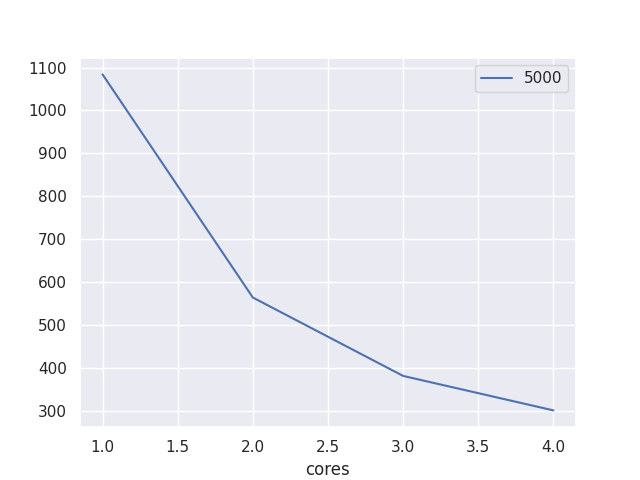
\includegraphics[width=0.7\linewidth]{plots/time-1}
		\caption[Time Plot]{Time plot. The y axis is the time in seconds while the x axis is the number of cores used. This is only for the 5000 sized matrix.}
		\label{fig:time-1}
	\end{figure}
	
\begin{figure}[H]
	\centering
	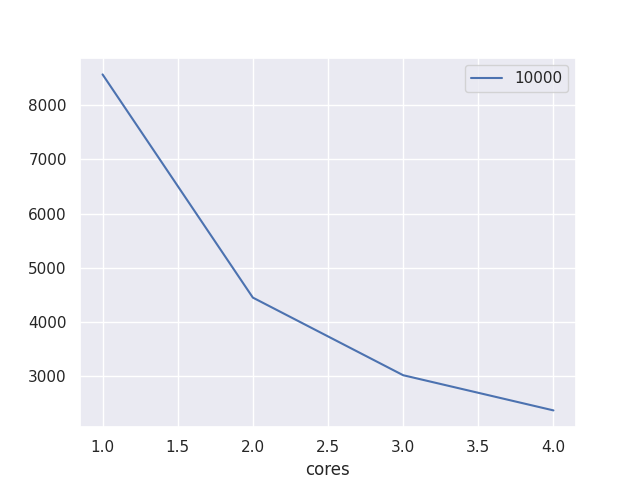
\includegraphics[width=0.7\linewidth]{plots/time-2}
	\caption[Time Plot]{Time plot. The y axis is the time in seconds while the x axis is the number of cores used. It contains the data from the 10000 sized matrix.}
	\label{fig:time-2}
\end{figure}
	
\begin{figure}[H]
	\centering
	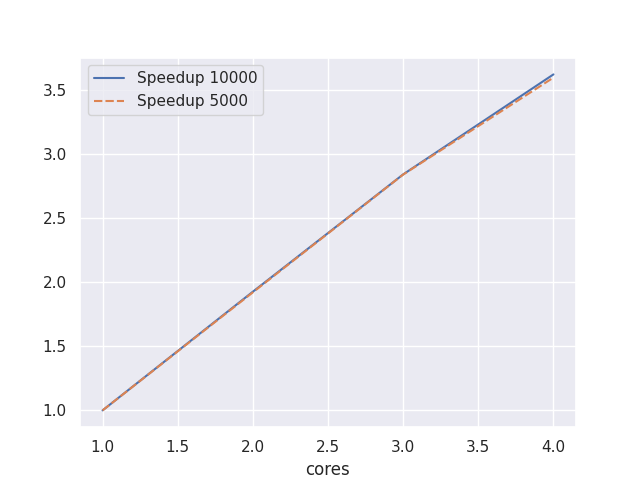
\includegraphics[width=0.7\linewidth]{plots/speedup}
	\caption[Speedup plot]{Speedup plot. The y axis is the speedup while the x axis is the number of cores used.}
	\label{fig:speedup}
\end{figure}
	
\begin{figure}[H]
	\centering
	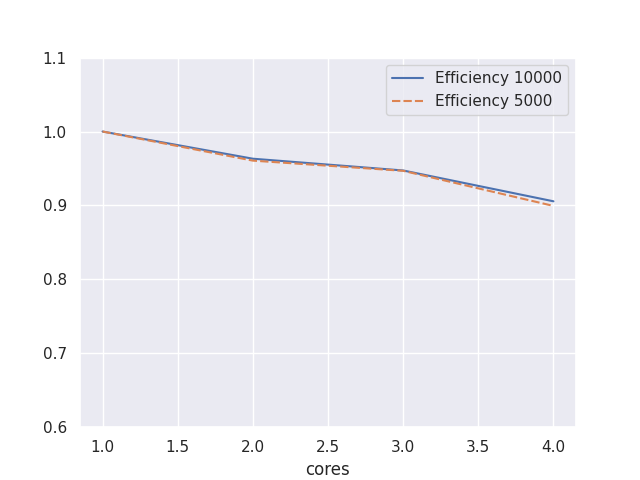
\includegraphics[width=0.7\linewidth]{plots/efficiency}
	\caption[Efficiency plot]{Efficiency plot. The y axis is the efficiency while the x axis is the number of cores used.}
	\label{fig:efficiency}
\end{figure}
	\subsection{Analysis}
	This application is almost embarrassingly parallel, as the costs and the speedup increase linearly with the number of cores that uses them. But, there is a small bottleneck that is reading the file: as the disc storage is not concurrent, the reading must be set to read in parallel. For this reason, it can be seen that the efficiency worsens in each core added, as that part of the program is sequential.\\
\\
This pattern can be seen more clearly at the efficiency plot, as the efficiency limits to the part of the code that can not be done concurrently, as shown in the next formula:
\[ \lim_{x \to \infty} \frac{T_s }{(T_{\text{read file}} +  \frac{T_p}{x}) \cdot x } = lim_{x \to \infty}\frac{T_s}{T_{\text{read file} \cdot x + T_p}} = 0\]
This means that the efficiency will eventually reach 0, as the time spend reading the file will never be parallelized. This also means that the maximum speed up is:
\[ \lim_{x \to \infty} \frac{T_s}{T_{\text{read file}} + T_p} = \frac{T_s}{T_{\text{read file}}}\]
\\
What's more, this pattern is shockingly the same with both benchmarks that were tried, where at two decimals precision, only with four cores there is a change between them in the efficiency. The aggregated difference in the speedup is also minimal, adding up to $0.3$.
	\section{Conclusion}
	In this project we parallelized the algorithm of the Game of Life, reaching almost embarrassingly parallel levels of concurrency in the program with the correct use of the scheduler and the optimizations in the GCC set to maximum\\
\\
Moreover, it was determined that the reading part of the game of life takes is the only sequential part of the whole operation, which makes the efficiency slow down as the number of cores rises when eventually it will reach 0. Additionally, the speedup is theoretically relative to the time spent reading the file.\\
\\

	

\end{document}
